\section{Kompilierung zu high-level Architekturen}

\begin{frame}{Wie ein Compiler den AST traversiert}
	\begin{figure}[h]
		\centering
		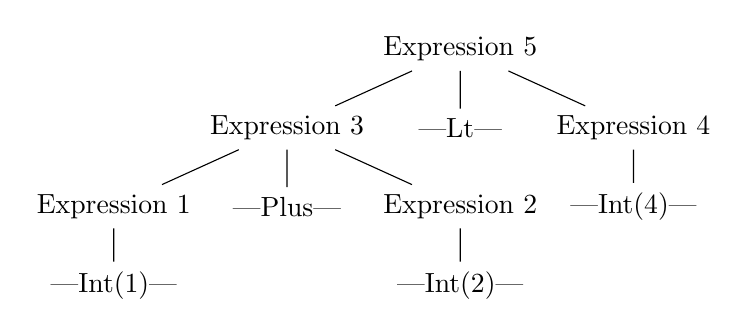
\begin{tikzpicture}[level distance=1cm, sibling distance=2.2cm]
			\node {Expression \encircle{5}}
			child {node {Expression \encircle{3}}
					child {node {Expression \encircle{1}}
							child {node {\Verb|Int(1)|}}}
					child {node {\Verb|Plus|}}
					child {node {Expression \encircle{2}}
							child {node {\Verb|Int(2)|}}}}
			child {node {\Verb|Lt|}}
			child {node {Expression \encircle{4}}
					child {node {\Verb|Int(4)|}}};
		\end{tikzpicture}
		\caption{AST zu \enquote{\texttt{1 + 2 < 4}}.}\label{fig:cmp_simple_tree}
	\end{figure}

	\Lirsting[raw=true, caption={Beispielausgabe zu \enquote{\texttt{1 + 2 < 4}}.}, label={lst:cmp_simple_instructions}, float=H]{deps/paper/listings/simple_compiler_instructions.txt}
\end{frame}
